\section{Course Overview}

Welcome! Please check Canvas for important announcements, materials, and links throughout the semester.
You'll also find course materials on Google Drive. Send me a request for access if the folder is not already shared with you. 

\smallskip
The point of the class is to learn Python \emph{for} \underline{data analysis}. 
This is not a computer science class and we will avoid taking too 
many detours that do not add meaningfully to a data analyst's/scientist's skillset. That means we'll learn 
enough syntax to manipulate data, analyze data, comfortably use existing packages, and write code for simple enough tasks where
there might not be a suitable function we can pull of the shelf.

\smallskip
We'll also be using Python 3. Syntax for Python 2 is slightly different, so don't be surprised if you find some
discrepancies in syntax in old Stack Exchange posts and in other resources. 


\subsection{Faculty}


\begin{lstlisting}[language = Python]
instructor, instructor_email = "Alexander Clark", "ac4725@columbia.edu"
# associate, associate_email = 
\end{lstlisting}

We're available by appointment and we'll set office hours based on the week.



\subsection{Books \& My Programming Lab}

To start, we're working from \emph{Starting out with Python} by Tony Gaddis. We'll use the accompanying My Programming Lab (MPL) exercises.
I'll have more to say about MPL later. My tentative plan is that MPL will be graded only to the requirement that you try half of the exercises.

\subsection{Software}

I think it's important we aren't dogmatic about the IDE or software we use, but you must download Anaconda. Contact me or the associate if you have trouble with the installation.
We'll work with Jupyter and Spyder. I also recommend you download Sublime Text or another simple text editor with synatax highlighting.
I will also use Google Colaboratory until we formally introduce Jupyter later in the course. 


\section{Why Python?}

First, what is Python? It's a high-level, general-purpose programming language. 
It is more general-purpose than a language like R. 
With libraries like pandas and scikit-learn available, it is now popular for data analysis.

Python's advantages over R are its readability and its popularity.

See the \link{https://www.python.org/dev/peps/pep-0020/}{Zen of Python} for design guidelines and \link{https://www.python.org/dev/peps/pep-0008/}{Pep 8} for a coding style guide.

You'll see Python in more job listings. I use Python every day, and I use R only occasionally for its more advanced statistical packages.

\begin{center}
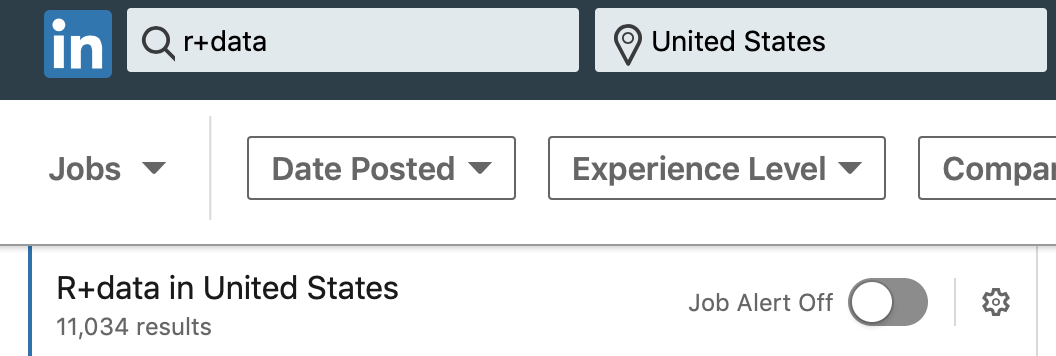
\includegraphics[width = .45\textwidth]{R_data_linkedin.png} 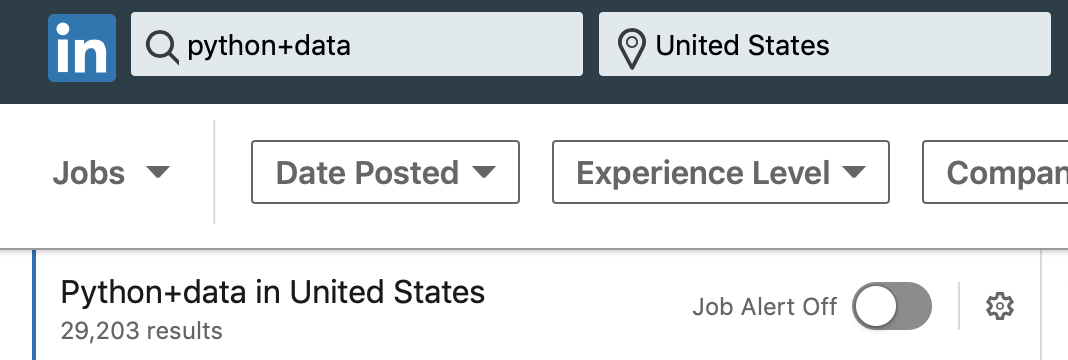
\includegraphics[width = .45\textwidth]{Python_data_linkedin.png}
\end{center}

\faMicrophone \faEyedropper.

\section{Input, Processing, and Output}
\scalebox{0.8}{\textit{Reference: Gaddis Chapter 2}}


\subsection{The Hello World Program (G\S 2.3)}

To get started in any langauge, printing ``Hello, World!'' might be the first step.\footnote{See
\textcolor{blue}{\href{https://en.wikipedia.org/wiki/\%22Hello,_World!\%22_program}
{the Wikipedia page for Hello, World.}}}

In Python, we can print an input using the \code{print()} function. We simply pass our
desired input within the parentheses, and Python will print the value.

We can enter text as a \textbf{string}. Text entered inside single, double, or triple quotations is interpreted as a string.


\begin{lstlisting}[language = Python]
print('Hello, World')
print("Hello, World!")
print("""Hello,
World!""") \end{lstlisting}


\smallskip
In Python 2, the syntax would have been \code{print 'Hello, World!'} without the parentheses.

\subsection{Comments (G\S 2.4)}

Commenting your code is helpful if you care about your colleagues or your future self. Comments should add clarity to
the intention and workings of code. A comment is a piece of code that isn't actually executed---it's a comment left for the reader or the person who inherits and modifies your code.
Everything after a \lstinline[language = Python]{#} will be ignored by the Python interpreter.

\begin{lstlisting}[language = Python]
# This will print a greeting.
print('Hello, World!') \end{lstlisting}

\smallskip
 You might also use end-line comments like the following

\begin{lstlisting}[language = Python]
print('Hello, World!') # Prints a greeting \end{lstlisting}

\smallskip

PEP 8 addresses comments \textcolor{blue}{\href{https://www.python.org/dev/peps/pep-0008/\#comments}{here}}.
I don't intend to grade based on the stylistic orthodoxy of your comments, but spaces are free so I do recommend 
\lstinline[language = Python]{# Comments like this} instead of \lstinline[language = Python]{#Comments like this}.


\subsection{Variables (G\S 2.5)}

A \textbf{variable} holds a value. It can be a string, a number, or perhaps a more complicated data type.
Variable assignment is done with the equals sign, \lstinline[language = Python]{=}.


\smallskip

\begin{lstlisting}[language = Python]
greeting = "Hello, World!"
my_favorite_number = 91 \end{lstlisting}

\smallskip

 Now compare the output you get from the following.

\begin{lstlisting}[language = Python]
print(greeting)
print('greeting')
print("Hello, World!")
print(91)
print(my_favorite_number)
print('my_favorite_number')
print("My favorite number is", my_favorite_number)
print("My favorite number is ", my_favorite_number) \end{lstlisting}


\smallskip

 PEP 8 addresses variable names \textcolor{blue}{\href{https://www.python.org/dev/peps/pep-0008/\#function-and-variable-names}{here}}.
Use lowercase and underscores.
This is good advice, but I don't see any reason to be too wedded to this. If you want to assign a matrix to a variable, 
it's reasonable to use an uppercase letter as the variable name. There, a math convention overrides a Python convention. Indeed, Gaddis is fine with uppercase (p. 43).

\smallskip

 More importantly, avoid Python key words in your variable names. \textcolor{blue}{\href{https://www.w3schools.com/python/python_ref_keywords.asp}
{Here}} is a list of keywords which have a specific meaning in code. An IDE will make this easier for you by highlighting keywords.

\begin{center}
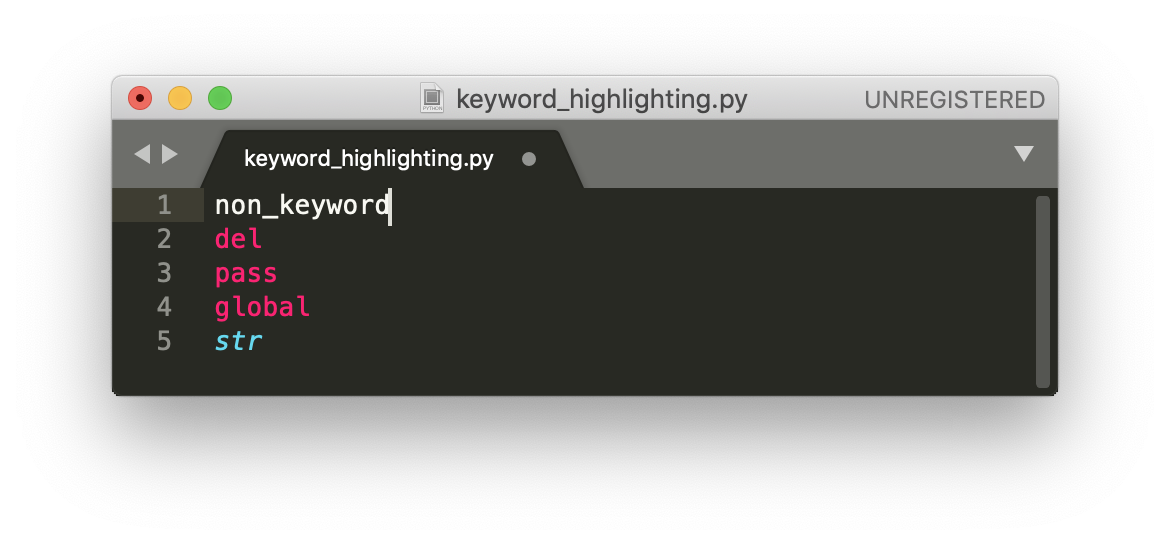
\includegraphics[width = .53\textwidth]{sublime_keyword_highlight.png}
\end{center}

\subsection{Data Types and Conversion (G\S 2.5, 2.6)}

To start, we are concerned with strings, integers, and floats. In Python, these are classes 
\lstinline{str}, \lstinline{int}, and \lstinline{float}.
You can check the type of variable or value using \lstinline[language = Python]{type()}.


\begin{lstlisting}[language = Python]
string_example = ''
int_example = -1
float_example = -1. \end{lstlisting}

\smallskip
 Some types can be converted by using \lstinline[language = Python]{str()},
\lstinline[language = Python]{int()}, or \lstinline[language = Python]{float()}.


\subsection{Input (G\S 2.6)}

It's not that common for a data science workflow, but you can read input using \lstinline[language = Python]{input()}.
The input is always read in as a string.

\begin{lstlisting}[language = Python]
favorte_color = input("What is your favorite color?")
favorite_number = input("What is your favorite number?")
attending_in_person = input("I am attending class in person.") \end{lstlisting}


\subsection{Calculations (G\S 2.7)}

You can use Python as a calculator. See the list of operations and symbols in Table 2-3 (Gaddis p. 54).
What might stand out is 
\begin{itemize}
\item Exponentiation is done with \lstinline[language = Python]{**}, not \lstinline[language = Python]{^}.
\item Integer division (rounds down) is done with \lstinline[language = Python]{//}.
\item The remainder of $x$ divided by $y$ can be found with \code{x \% y}, which might be read as
$x$ \emph{modulo} $y$. 
\end{itemize}

If a float is involved in an operation, the result will also be a float. 


\section{Decision Structures}
\scalebox{0.8}{\textit{Reference: Gaddis Chapter 3}}

Decision structures allow a program to have more than one path of execution. The path depends on condition. The condition is either True or False, and so can be represented by a Boolean variable.

\subsection{If Statements (G\S 3.1, 3.3)}

Here's a joke. A programmer is going to the grocery store and his partner says, ``Buy a gallon of milk, and if there are eggs, buy a dozen.''
The programmer comes home with 13 gallons of milk.

Or consider the logical inference if you ask, ``Is it raining?'' and get a reply, ``Not hard.'' 


\begin{lstlisting}[language = Python]
if 2 + 2 > 4:
    print("Pigs can fly.")
    
if 2 + 2 == 4:
    print("Pigs cannot fly.")
    
if 'a' < 'b':
    print("It is true that 'a' is less than 'b'.")
    
if 'a' < 'A':
    print("It is true that 'a' is less than 'A'.")
    
if 'goon' == 'Goblin':
    print("A goon is a goblin.") \end{lstlisting}
    
%https://genius.com/annotations/2257/standalone_embed

If statements like the above rely on \emph{relational operators} (see Table 3-1 Gaddis p.112).

\begin{lstlisting}[language = Python]
if 2 == 2.:
    print("The integer and the float are equal.")
    
if 2 is 2.:
    print("The integer and the float are the same object in memory.") \end{lstlisting}

\subsection{If Elif Else Statements (G\S 3.2, 3.4)}

Compare the output from the following programs.

\begin{lstlisting}[language = Python]
num = 0

if num < 1:
    print(num)
    num = num + 2
if num > 0:
    print(num, '!')
    num = num - 1000
if True:
    print(num, '?') \end{lstlisting}


\begin{lstlisting}[language = Python]
num = 0

if num < 1:
    print(num)
    num = num + 2
elif num > 0:
    print(num, '!')
    num = num - 1000
else:
    print(num, '?') \end{lstlisting}


\subsection{Logical Operators (G\S 3.5)}

Suppose you want to execute some code if a number $x$ is between 10 and 20. You could use \emph{nested} if statements.
\begin{lstlisting}[language = Python]
x = 14
if x >= 10:
    if x <= 20:
        print("x is between 10 and 20.") \end{lstlisting}
        

\smallskip
 But you might prefer to base your if statement off of one compound Boolean expression. For these, we need logical operations. They are

\begin{itemize}

\item Logical \textit{and}: \code{and} %, \lstinline[language = Python]{&}
\item Logical \textit{or}: \code{or} %, \lstinline[language = Python]{|}
\item Logical \textit{negation}: \code{not}
\end{itemize}
\smallskip

Observe the following will give equivalent output.

\begin{lstlisting}[language = Python]
not 1 > 2
not (1 > 2)
not(1 > 2) \end{lstlisting}


\smallskip

 \textbf{Challenge: } What do you expect from \lstinline[language = Python]{not not (1 or False)}?
        


\subsection{Boolean Variables (G\S 3.6)}

Finally, a Boolean variable simply references a logical True or False.

\begin{lstlisting}[language = Python]
# Option Value
market_value = 10
strike_price = 9
option_has_value = market_value > strike_price

if option_has_value:
    print("We're in the money.")
    
# Check data type
print(type(option_has_value)
print(type(False))) \end{lstlisting}